\subsection{Beispiel: Lineare Regression}\label{maschinelleslernen:linregress}
Beispiel aus dem Bereich Regression. Konkret wird hier eine lineare Regression dargestellt. 

Es \randnotiz{Importe}sind verschiedene Importe f�r n�tig. Die werden im ersten Schritt importiert.
\lstinputlisting[language=Python,firstline=1,lastline=5]{chapters/advancedTopics/src/machinelearning/linregress.py}\label{knnsample:lst:lingress1}

Daten \randnotiz{Daten laden}aus dem Datensatz \lstinline$boston$ auslesen und in \lstinline$numpy-array$ �berf�hren.
\lstinputlisting[language=Python,firstline=7,lastline=10]{chapters/advancedTopics/src/machinelearning/linregress.py}\label{knnsample:lst:lingress7}

Die \randnotiz{Berechnung durchf�hren}Berechnung der linearen Regression kann direkt aus dem Modul \lstinline$scipy$ erfolgen, es ist keine eigene Implementierung n�tig. Die Daten die analysiert werden sollen m�ssen entsprechend mitgegeben werden.
\lstinputlisting[language=Python,firstline=12,lastline=13]{chapters/advancedTopics/src/machinelearning/linregress.py}\label{knnsample:lst:lingress12}

Nun \randnotiz{Plot erzeugen}kann der Plot f�r die berechneten Werte erzeugt werden.
\lstinputlisting[language=Python,firstline=15,lastline=27]{chapters/advancedTopics/src/machinelearning/linregress.py}\label{knnsample:lst:lingress15}

Die Anzeige im Plot ist wie in Abbildung ~\ref{ml:samples:plotlinregress}.

\begin{figure}[ht]
	\centering
	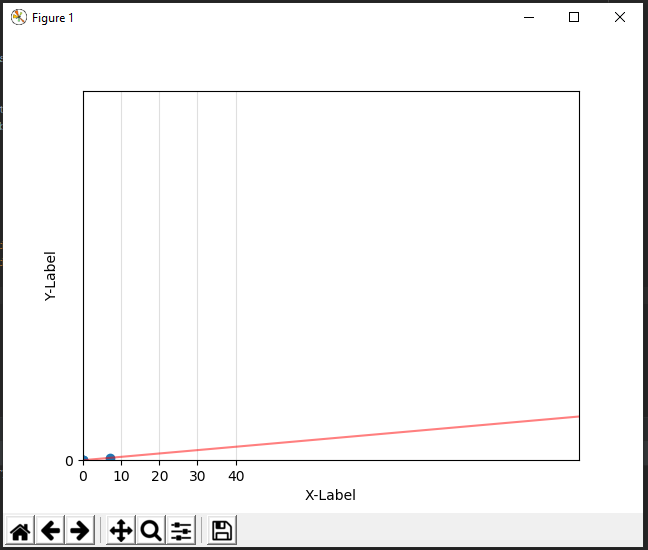
\includegraphics[width=0.9\textwidth]{images/MachineLearning/ml_linregress_plot.png}
	\caption{Ergebnis-Plot der linearen Regression}
	\label{ml:samples:plotlinregress}
\end{figure}

Somit haben wir nun auch eine lineare Regression erfolgreich durchgef�hrt.


\uebung
\aufgabe{MachineLearning/machinelearning_linregress}